\chapter{Ordenação}

\index{Ordenação}

\key{Ordenação}
é um problema fundamental no design de algoritmos.
Muitos algoritmos eficientes
utilizam a ordenação como uma sub-rotina, 
pois frequentemente é mais fácil processar 
os dados quando os elementos estão ordenados.

Por exemplo, o problema ''um array contém 
dois elementos iguais?'' é fácil de resolver usando ordenação. 
Se o array contiver dois elementos iguais, 
eles estarão um ao lado do outro após a ordenação, 
então é fácil encontrá-los. 
Além disso, o problema ''qual é o elemento mais frequente
 em um array?'' pode ser resolvido de forma semelhante.

Existem muitos algoritmos para ordenação, e eles também são
bons exemplos de como aplicar 
diferentes técnicas de design de algoritmos. 
Os algoritmos de ordenação eficientes
funcionam em tempo $O(n \log n)$, 
e muitos algoritmos que usam a ordenação
como sub-rotina também 
têm essa complexidade de tempo.

\section{Teoria da ordenação}

O problema básico na ordenação é o seguinte:
\begin{framed}
\noindent
Dado um array que contém $n$ elementos,
sua tarefa é ordenar os elementos 
em ordem crescente.
\end{framed}
\noindent
Por exemplo, o array
\begin{center}
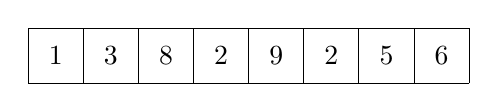
\begin{tikzpicture}[scale=0.7]
\draw (0,0) grid (8,1);
\node at (0.5,0.5) {$1$};
\node at (1.5,0.5) {$3$};
\node at (2.5,0.5) {$8$};
\node at (3.5,0.5) {$2$};
\node at (4.5,0.5) {$9$};
\node at (5.5,0.5) {$2$};
\node at (6.5,0.5) {$5$};
\node at (7.5,0.5) {$6$};
\end{tikzpicture}
\end{center}
ficará da seguinte forma após a ordenação:
\begin{center}
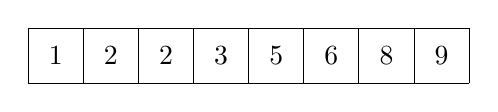
\begin{tikzpicture}[scale=0.7]
\draw (0,0) grid (8,1);
\node at (0.5,0.5) {$1$};
\node at (1.5,0.5) {$2$};
\node at (2.5,0.5) {$2$};
\node at (3.5,0.5) {$3$};
\node at (4.5,0.5) {$5$};
\node at (5.5,0.5) {$6$};
\node at (6.5,0.5) {$8$};
\node at (7.5,0.5) {$9$};
\end{tikzpicture}
\end{center}

\subsubsection{Algoritmos $O(n^2)$}

\index{bubble sort}

Algoritmos simples para ordenar um array
operam em tempo $O(n^2)$.
Tais algoritmos são curtos e geralmente
consistem em dois loops aninhados.
Um famoso algoritmo de ordenação em tempo $O(n^2)$
é o \key{bubble sort} onde os elementos
"flutuam" no array de acordo com seus valores.

O Bubble sort consiste em $n$ rodadas.
Em cada rodada, o algoritmo percorre
os elementos do array.
Sempre que dois elementos consecutivos são encontrados
que não estão na ordem correta,
o algoritmo os troca.
O algoritmo pode ser implementado da seguinte forma:
\begin{lstlisting}
for (int i = 0; i < n; i++) {
    for (int j = 0; j < n-1; j++) {
        if (array[j] > array[j+1]) {
            swap(array[j],array[j+1]);
        }
    }
}
\end{lstlisting}

Após a primeira rodada do algoritmo,
o maior elemento estará na posição correta,
e em geral, após $k$ rodadas, os $k$ maiores
elementos estarão nas posições corretas.
Portanto, após $n$ rodadas, o array inteiro
estará ordenado.

Por exemplo, no array

\begin{center}
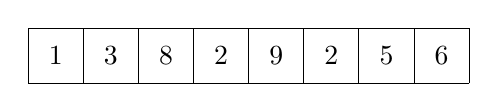
\begin{tikzpicture}[scale=0.7]
\draw (0,0) grid (8,1);

\node at (0.5,0.5) {$1$};
\node at (1.5,0.5) {$3$};
\node at (2.5,0.5) {$8$};
\node at (3.5,0.5) {$2$};
\node at (4.5,0.5) {$9$};
\node at (5.5,0.5) {$2$};
\node at (6.5,0.5) {$5$};
\node at (7.5,0.5) {$6$};
\end{tikzpicture}
\end{center}

\noindent
na primeira rodada do bubble sort, os elementos
são trocados da seguinte forma:

\begin{center}
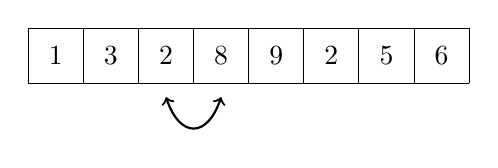
\begin{tikzpicture}[scale=0.7]
\draw (0,0) grid (8,1);
\node at (0.5,0.5) {$1$};
\node at (1.5,0.5) {$3$};
\node at (2.5,0.5) {$2$};
\node at (3.5,0.5) {$8$};
\node at (4.5,0.5) {$9$};
\node at (5.5,0.5) {$2$};
\node at (6.5,0.5) {$5$};
\node at (7.5,0.5) {$6$};

\draw[thick,<->] (3.5,-0.25) .. controls (3.25,-1.00) and (2.75,-1.00) .. (2.5,-0.25);
\end{tikzpicture}
\end{center}

\begin{center}
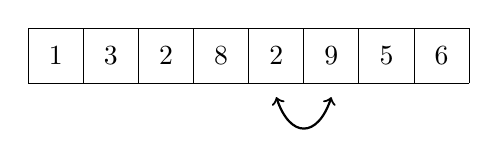
\begin{tikzpicture}[scale=0.7]
\draw (0,0) grid (8,1);
\node at (0.5,0.5) {$1$};
\node at (1.5,0.5) {$3$};
\node at (2.5,0.5) {$2$};
\node at (3.5,0.5) {$8$};
\node at (4.5,0.5) {$2$};
\node at (5.5,0.5) {$9$};
\node at (6.5,0.5) {$5$};
\node at (7.5,0.5) {$6$};

\draw[thick,<->] (5.5,-0.25) .. controls (5.25,-1.00) and (4.75,-1.00) .. (4.5,-0.25);
\end{tikzpicture}
\end{center}

\begin{center}
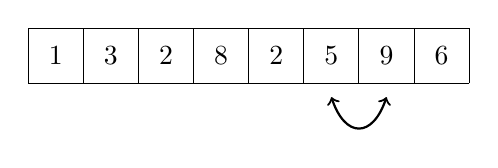
\begin{tikzpicture}[scale=0.7]
\draw (0,0) grid (8,1);
\node at (0.5,0.5) {$1$};
\node at (1.5,0.5) {$3$};
\node at (2.5,0.5) {$2$};
\node at (3.5,0.5) {$8$};
\node at (4.5,0.5) {$2$};
\node at (5.5,0.5) {$5$};
\node at (6.5,0.5) {$9$};
\node at (7.5,0.5) {$6$};

\draw[thick,<->] (6.5,-0.25) .. controls (6.25,-1.00) and (5.75,-1.00) .. (5.5,-0.25);
\end{tikzpicture}
\end{center}

\begin{center}
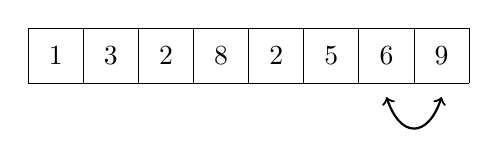
\begin{tikzpicture}[scale=0.7]
\draw (0,0) grid (8,1);
\node at (0.5,0.5) {$1$};
\node at (1.5,0.5) {$3$};
\node at (2.5,0.5) {$2$};
\node at (3.5,0.5) {$8$};
\node at (4.5,0.5) {$2$};
\node at (5.5,0.5) {$5$};
\node at (6.5,0.5) {$6$};
\node at (7.5,0.5) {$9$};

\draw[thick,<->] (7.5,-0.25) .. controls (7.25,-1.00) and (6.75,-1.00) .. (6.5,-0.25);
\end{tikzpicture}
\end{center}

\subsubsection{Inversões}

\index{inversão}

O Bubble sort é um exemplo de um algoritmo de ordenação
que sempre troca elementos \emph{consecutivos} no array.
Acontece que a complexidade de tempo de tal algoritmo é \emph{sempre}
pelo menos $O(n^2)$, porque no pior caso, são necessárias,
$O(n^2)$ trocas para ordenar o array.

Um conceito útil ao analisar algoritmos de ordenação é uma \key{inversão}:
um par de elementos de array
$(\texttt{array}[a],\texttt{array}[b])$ tal que
$a<b$ and $\texttt{array}[a]>\texttt{array}[b]$,
ou seja, os elementos estão na ordem errada. 
Por exemplo, o array
\begin{center}
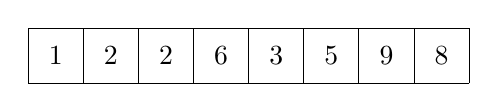
\begin{tikzpicture}[scale=0.7]
\draw (0,0) grid (8,1);
\node at (0.5,0.5) {$1$};
\node at (1.5,0.5) {$2$};
\node at (2.5,0.5) {$2$};
\node at (3.5,0.5) {$6$};
\node at (4.5,0.5) {$3$};
\node at (5.5,0.5) {$5$};
\node at (6.5,0.5) {$9$};
\node at (7.5,0.5) {$8$};
\end{tikzpicture}
\end{center}
tem três inversões: $(6,3)$, $(6,5)$ and $(9,8)$.
O número de inversões indica o quanto de trabalho é necessário para ordenar o array. 
Um array está completamente ordenado quando não há inversões.
Por outro lado, se os elementos do array estiverem em ordem reversa, o número de inversões é o máximo possível:
\[1+2+\cdots+(n-1)=\frac{n(n-1)}{2} = O(n^2)\]

A troca de um par de elementos consecutivos que estão na ordem errada remove exatamente uma inversão do array.
Portanto, se um algoritmo de ordenação só pode trocar elementos consecutivos, cada troca remove no máximo uma inversão, e a complexidade de tempo do algoritmo é pelo menos $O(n^2)$.

\subsubsection{Algoritmos $O(n \log n)$}

\index{merge sort}

É possível ordenar um array de forma eficiente em
tempo $O(n \log n)$ usando algoritmos que não estão limitados a trocar elementos consecutivos.
Um desses algoritmos é o \key{merge sort}\footnote{De acordo com \cite{knu983},
o merge sort foi inventado por J. von Neumann em 1945.},
que é baseado em recursão.


Merge sort ordena um subarray \texttt{array}$[a \ldots b]$ da seguinte forma:

\begin{enumerate}
\item Se $a=b$, não faça nada, pois o subarray já está ordenado..
\item Calcule a posição do elemento do meio: $k=\lfloor (a+b)/2 \rfloor$.
\item Ordene recursivamente o subarray \texttt{array}$[a \ldots k]$.
\item Ordene recursivamente o subarray \texttt{array}$[k+1 \ldots b]$.
\item \emph{Junte} os subarrays ordenados \texttt{array}$[a \ldots k]$ e
\texttt{array}$[k+1 \ldots b]$
em um subarray ordenado \texttt{array}$[a \ldots b]$.
\end{enumerate}

O merge sort é um algoritmo eficiente porque ele reduz pela metade o tamanho do subarray a cada passo.
A recursão consiste em $O(\log n)$ níveis,
e processar cada nível leva tempo $O(n)$.
Juntar os subarrays \texttt{array}$[a \ldots k]$ e \texttt{array}$[k+1 \ldots b]$
é possível em tempo linear, porque eles já estão ordenados.

Por exemplo, considere ordenar o seguinte array:
\begin{center}
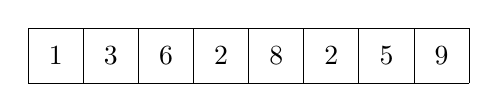
\begin{tikzpicture}[scale=0.7]
\draw (0,0) grid (8,1);
\node at (0.5,0.5) {$1$};
\node at (1.5,0.5) {$3$};
\node at (2.5,0.5) {$6$};
\node at (3.5,0.5) {$2$};
\node at (4.5,0.5) {$8$};
\node at (5.5,0.5) {$2$};
\node at (6.5,0.5) {$5$};
\node at (7.5,0.5) {$9$};
\end{tikzpicture}
\end{center}

O array será dividido em dois subarrays da seguinte forma:
\begin{center}
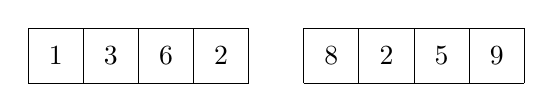
\begin{tikzpicture}[scale=0.7]
\draw (0,0) grid (4,1);
\draw (5,0) grid (9,1);

\node at (0.5,0.5) {$1$};
\node at (1.5,0.5) {$3$};
\node at (2.5,0.5) {$6$};
\node at (3.5,0.5) {$2$};

\node at (5.5,0.5) {$8$};
\node at (6.5,0.5) {$2$};
\node at (7.5,0.5) {$5$};
\node at (8.5,0.5) {$9$};
\end{tikzpicture}
\end{center}

Então, os subarrays serão ordenados recursivamente da seguinte forma:
\begin{center}
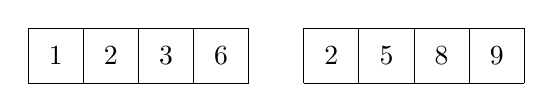
\begin{tikzpicture}[scale=0.7]
\draw (0,0) grid (4,1);
\draw (5,0) grid (9,1);

\node at (0.5,0.5) {$1$};
\node at (1.5,0.5) {$2$};
\node at (2.5,0.5) {$3$};
\node at (3.5,0.5) {$6$};

\node at (5.5,0.5) {$2$};
\node at (6.5,0.5) {$5$};
\node at (7.5,0.5) {$8$};
\node at (8.5,0.5) {$9$};
\end{tikzpicture}
\end{center}

Finalmente, o algoritmo junta os subarrays ordenados e cria o array final ordenado:
\begin{center}
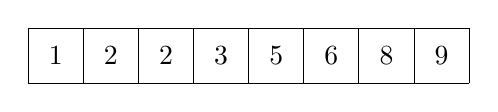
\begin{tikzpicture}[scale=0.7]
\draw (0,0) grid (8,1);
\node at (0.5,0.5) {$1$};
\node at (1.5,0.5) {$2$};
\node at (2.5,0.5) {$2$};
\node at (3.5,0.5) {$3$};
\node at (4.5,0.5) {$5$};
\node at (5.5,0.5) {$6$};
\node at (6.5,0.5) {$8$};
\node at (7.5,0.5) {$9$};
\end{tikzpicture}
\end{center}

\subsubsection{Limite Inferior de Ordenação}

É possível ordenar um array mais rápido
do que em tempo $O(n \log n)$?
Acontece que isso \emph{não} é possível
quando nos limitamos a algoritmos de ordenação baseados na comparação de elementos do array.

O limite inferior para a complexidade temporal
pode ser demonstrado considerando a ordenação
como um processo no qual cada comparação de dois elementos fornece mais informações sobre o conteúdo do array.
O processo cria a seguinte árvore:

\begin{center}
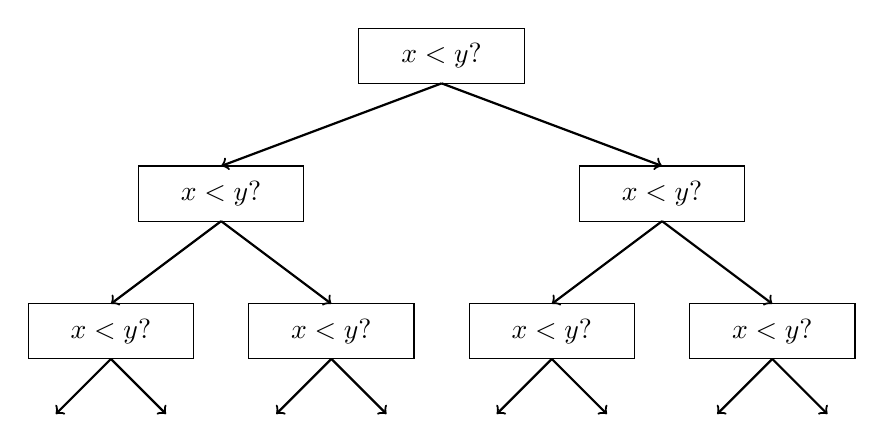
\begin{tikzpicture}[scale=0.7]
\draw (0,0) rectangle (3,1);
\node at (1.5,0.5) {$x < y?$};

\draw[thick,->] (1.5,0) -- (-2.5,-1.5);
\draw[thick,->] (1.5,0) -- (5.5,-1.5);

\draw (-4,-2.5) rectangle (-1,-1.5);
\draw (4,-2.5) rectangle (7,-1.5);
\node at (-2.5,-2) {$x < y?$};
\node at (5.5,-2) {$x < y?$};

\draw[thick,->] (-2.5,-2.5) -- (-4.5,-4);
\draw[thick,->] (-2.5,-2.5) -- (-0.5,-4);
\draw[thick,->] (5.5,-2.5) -- (3.5,-4);
\draw[thick,->] (5.5,-2.5) -- (7.5,-4);

\draw (-6,-5) rectangle (-3,-4);
\draw (-2,-5) rectangle (1,-4);
\draw (2,-5) rectangle (5,-4);
\draw (6,-5) rectangle (9,-4);
\node at (-4.5,-4.5) {$x < y?$};
\node at (-0.5,-4.5) {$x < y?$};
\node at (3.5,-4.5) {$x < y?$};
\node at (7.5,-4.5) {$x < y?$};

\draw[thick,->] (-4.5,-5) -- (-5.5,-6);
\draw[thick,->] (-4.5,-5) -- (-3.5,-6);
\draw[thick,->] (-0.5,-5) -- (0.5,-6);
\draw[thick,->] (-0.5,-5) -- (-1.5,-6);
\draw[thick,->] (3.5,-5) -- (2.5,-6);
\draw[thick,->] (3.5,-5) -- (4.5,-6);
\draw[thick,->] (7.5,-5) -- (6.5,-6);
\draw[thick,->] (7.5,-5) -- (8.5,-6);
\end{tikzpicture}
\end{center}

Aqui ''$x<y?$'' significa que alguns elementos
$x$ e $y$ são comparados.
Se $x<y$, o processo continua para a esquerda e,
caso contrário, para a direita.
Os resultados do processo são as possíveis
maneiras de ordenar o array, um total de $n!$ maneiras.
Por essa razão, a altura da árvore deve ser pelo menos
\[ \log_2(n!) = \log_2(1)+\log_2(2)+\cdots+\log_2(n).\]
Obtemos um limite inferior para esta soma
escolhendo os últimos $n/2$ elementos e
alterando o valor de cada elemento para $\log_2(n/2)$.
Isso nos dá uma estimativa
\[ \log_2(n!) \ge (n/2) \cdot \log_2(n/2),\]
portanto, a altura da árvore e o número mínimo possível de etapas em um algoritmo de ordenação no pior caso é pelo menos $n \log n$.

\subsubsection{Counting sort}

\index{counting sort}

O limite inferior $n \log n$ não se aplica a algoritmos que não comparam elementos de array, mas usam alguma outra informação. Um exemplo de tal algoritmo é o
\key{counting sort} que ordena um array em tempo
$O(n)$ assumindo que cada elemento no array é um inteiro entre $0 \ldots c$ e $c=O(n)$.

O algoritmo cria um \emph{array de contagem},
cujos índices são elementos do array original.
O algoritmo itera pelo array original e calcula quantas vezes cada elemento aparece no array.
\newpage

Por exemplo, o array
\begin{center}
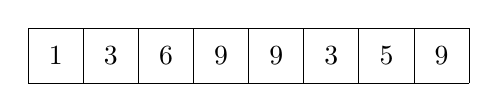
\begin{tikzpicture}[scale=0.7]
\draw (0,0) grid (8,1);
\node at (0.5,0.5) {$1$};
\node at (1.5,0.5) {$3$};
\node at (2.5,0.5) {$6$};
\node at (3.5,0.5) {$9$};
\node at (4.5,0.5) {$9$};
\node at (5.5,0.5) {$3$};
\node at (6.5,0.5) {$5$};
\node at (7.5,0.5) {$9$};
\end{tikzpicture}
\end{center}
corresponde ao array de contagem a seguir:
\begin{center}
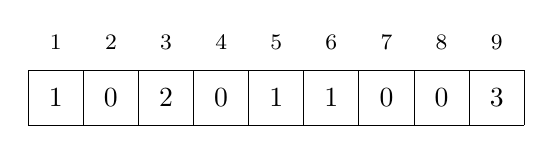
\begin{tikzpicture}[scale=0.7]
\draw (0,0) grid (9,1);
\node at (0.5,0.5) {$1$};
\node at (1.5,0.5) {$0$};
\node at (2.5,0.5) {$2$};
\node at (3.5,0.5) {$0$};
\node at (4.5,0.5) {$1$};
\node at (5.5,0.5) {$1$};
\node at (6.5,0.5) {$0$};
\node at (7.5,0.5) {$0$};
\node at (8.5,0.5) {$3$};

\footnotesize

\node at (0.5,1.5) {$1$};
\node at (1.5,1.5) {$2$};
\node at (2.5,1.5) {$3$};
\node at (3.5,1.5) {$4$};
\node at (4.5,1.5) {$5$};
\node at (5.5,1.5) {$6$};
\node at (6.5,1.5) {$7$};
\node at (7.5,1.5) {$8$};
\node at (8.5,1.5) {$9$};
\end{tikzpicture}
\end{center}

Por exemplo, o valor na posição 3
no array de contagem é 2,
porque o elemento 3 aparece 2 vezes
no array original.

A construção do array de contagem leva
tempo $O(n)$. Depois disso, o array ordenado pode ser criado em tempo $O(n)$ porque o número de ocorrências de cada elemento pode ser recuperado do array de contagem.
Portanto, a complexidade temporal total do counting sort é $O(n)$.

O counting sort é um algoritmo muito eficiente, mas só pode ser usado quando a constante $c$
é pequena o suficiente, de modo que os elementos do array
possam ser usados como índices no array de contagem.

\section{Ordenação em C++}

\index{sort@\texttt{sort}}

Quase nunca é uma boa ideia usar um algoritmo de ordenação feito em casa em uma competição, porque existem boas implementações disponíveis em linguagens de programação.
Por exemplo, a biblioteca padrão de C++ contém a função \texttt{sort} que pode ser facilmente usada para ordenar arrays e outras estruturas de dados.

Há muitos benefícios em usar uma função de biblioteca. Primeiro, isso economiza tempo porque não há necessidade de implementar a função. Segundo, a implementação da biblioteca é certamente correta e eficiente: é improvável que uma função de ordenação feita em casa seja melhor.

Nesta seção, veremos como usar a função \texttt{sort} em C++.
O código a seguir ordena um vetor em ordem crescente:
\begin{lstlisting}
vector<int> v = {4,2,5,3,5,8,3};
sort(v.begin(),v.end());
\end{lstlisting}
Após a ordenação, o conteúdo do vetor será:
$[2,3,3,4,5,5,8]$.
A ordem de classificação padrão é crescente, mas uma ordem reversa é possível da seguinte forma:
\begin{lstlisting}
sort(v.rbegin(),v.rend());
\end{lstlisting}
Um array comum pode ser ordenado da seguinte forma:
\begin{lstlisting}
int n = 7; // tamanho do array
int a[] = {4,2,5,3,5,8,3};
sort(a,a+n);
\end{lstlisting}
\newpage
O seguinte código ordena a string \texttt{s}:
\begin{lstlisting}
string s = "monkey";
sort(s.begin(), s.end());
\end{lstlisting}
Ordenar uma string significa que os caracteres da string são ordenados.
Por exemplo, a string ''monkey'' se torna ''ekmnoy''.

\subsubsection{Operadores de comparação}

\index{operador de comparação}

A função \texttt{sort} requer que um \key{operador de comparação} seja definido para o tipo de dados
dos elementos a serem ordenados.
Ao ordenar, esse operador será usado sempre que for necessário determinar a ordem de dois elementos.

A maioria dos tipos de dados em C++ tem um operador de comparação integrado, e elementos desses tipos podem ser ordenados automaticamente. Por exemplo, números são ordenados de acordo com seus valores e strings são ordenadas em ordem alfabética.

\index{pair@\texttt{pair}}

Pares (\texttt{pair}) são ordenados principalmente de acordo com seus primeiros elementos (\texttt{first}).
No entanto, se os primeiros elementos de dois pares forem iguais, eles são ordenados de acordo com seus segundos elementos (\texttt{second}):
\begin{lstlisting}
vector<pair<int,int>> v;
v.push_back({1,5});
v.push_back({2,3});
v.push_back({1,2});
sort(v.begin(), v.end());
\end{lstlisting}
Após isso, a ordem dos pares é:
$(1,2)$, $(1,5)$ and $(2,3)$.

\index{tuple@\texttt{tuple}}

De forma semelhante, tuplas (\texttt{tuple})
são ordenadas principalmente pelo primeiro elemento,
secundariamente pelo segundo elemento, etc.\footnote{Note que em alguns compiladores mais antigos, a função \texttt{make\_tuple} deve ser usada para criar uma tupla em vez de chaves (por exemplo, \texttt{make\_tuple(2,1,4)} em vez de \texttt{\{2,1,4\}}).}:
\begin{lstlisting}
vector<tuple<int,int,int>> v;
v.push_back({2,1,4});
v.push_back({1,5,3});
v.push_back({2,1,3});
sort(v.begin(), v.end());
\end{lstlisting}
Após isso, a ordem das tuplas é:
$(1,5,3)$, $(2,1,3)$ e $(2,1,4)$.

\subsubsection{Structs definidas pelo usuário}

As structs definidas pelo usuário não possuem um operador de comparação automaticamente.
O operador deve ser definido dentro da struct como uma função
\texttt{operator<},
cujo parâmetro é outro elemento do mesmo tipo.
O operador deve retornar \texttt{true}
se o elemento for menor que o parâmetro,
e \texttt{false} caso contrário.

Por exemplo, a seguinte struct \texttt{P}
contém as coordenadas x e y de um ponto.
O operador de comparação é definido de forma que os pontos sejam ordenados principalmente pela coordenada x e secundariamente pela coordenada y.

\begin{lstlisting}
struct P {
    int x, y;
    bool operator<(const P &p) {
        if (x != p.x) return x < p.x;
        else return y < p.y;
    }
};
\end{lstlisting}

\subsubsection{Funções de comparação}

\index{função de comparação}

Também é possível fornecer uma \key{função de comparação} externa para a função \texttt{sort} como uma função de callback. Por exemplo, a seguinte função de comparação \texttt{comp} ordena strings principalmente por comprimento e secundariamente por ordem alfabética:

\begin{lstlisting}
bool comp(string a, string b) {
    if (a.size() != b.size()) return a.size() < b.size();
    return a < b;
}
\end{lstlisting}
Agora um vetor de strings pode ser ordenado da seguinte forma:
\begin{lstlisting}
sort(v.begin(), v.end(), comp);
\end{lstlisting}

\section{Busca binária}

\index{busca binária}

Um método geral para buscar um elemento em um array é usar um loop \texttt{for}
que itera pelos elementos do array.
Por exemplo, o seguinte código busca por um elemento $x$ no array:

\begin{lstlisting}
for (int i = 0; i < n; i++) {
    if (array[i] == x) {
        // x encontrado no indice i
    }
}
\end{lstlisting}

A complexidade temporal desta abordagem é $O(n)$,
porque no pior caso é necessário verificar todos os elementos do array.
Se a ordem dos elementos for arbitrária, esta também é a melhor abordagem possível, pois não há informações adicionais disponíveis sobre onde no array devemos procurar pelo elemento $x$.

No entanto, se o array estiver \emph{ordenado},
a situação é diferente.
Neste caso, é possível realizar a busca muito mais rapidamente, porque a ordem dos elementos no array orienta a busca.
O seguinte algoritmo de \key{busca binária}
efetua a busca por um elemento em um array ordenado de forma eficiente em
tempo $O(\log n)$.

\subsubsection{Método 1}

A maneira usual de implementar a busca binária se assemelha a procurar uma palavra em um dicionário. A busca mantém uma região ativa no array, que inicialmente contém todos os elementos do array. Em seguida, um número de passos é executado, cada um dos quais divide pela metade o tamanho da região.

Em cada etapa, a busca verifica o elemento do meio da região ativa. Se o elemento do meio for o elemento alvo, a busca termina. Caso contrário, a busca continua recursivamente para a metade esquerda ou direita da região, dependendo do valor do elemento do meio.

A ideia acima pode ser implementada da seguinte forma:
\begin{lstlisting}
int a = 0, b = n-1;
while (a <= b) {
    int k = (a+b)/2;
    if (array[k] == x) {
        // x encontrado no indice k
    }
    if (array[k] > x) b = k-1;
    else a = k+1;
}
\end{lstlisting}

Nesta implementação, a região ativa é $a \ldots b$,
e inicialmente a região é $0 \ldots n-1$.
O algoritmo divide o tamanho da região pela metade a cada etapa,
então a complexidade temporal é $O(\log n)$.

\subsubsection{Método 2}

Um método alternativo para implementar a busca binária é baseado em uma maneira eficiente de iterar pelos elementos do array.
A ideia é fazer saltos e diminuir a velocidade quando estivermos mais perto do elemento alvo.

 busca percorre o array da esquerda para a direita, e o comprimento inicial do salto é $n/2$.
Em cada etapa, o comprimento do salto será dividido pela metade:
primeiro $n/4$, depois $n/8$, $n/16$, etc., até que finalmente o comprimento seja 1.
Após os saltos, ou o elemento alvo foi encontrado ou sabemos que ele não aparece no array.

O código a seguir implementa a ideia acima:
\begin{lstlisting}
int k = 0;
for (int b = n/2; b >= 1; b /= 2) {
    while (k+b < n && array[k+b] <= x) k += b;
}
if (array[k] == x) {
    // x encontrado no indice k
}
\end{lstlisting}

Durante a busca, a variável $b$
contém o comprimento atual do salto..
A complexidade temporal do algoritmo é $O(\log n)$,
porque o código no loop \texttt{while}
é executado no máximo duas vezes para cada comprimento de salto.

\subsubsection{Funções em C++}

A biblioteca padrão de C++ contém as seguintes funções que são baseadas em busca binária e funcionam em tempo logarítmico:

\begin{itemize}
\item \texttt{lower\_bound} retorna um ponteiro para o primeiro elemento do array cujo valor é pelo menos $x$.
\item \texttt{upper\_bound} retorna um ponteiro para o primeiro elemento do array cujo valor é maior do que $x$.
\item \texttt{equal\_range} retorna ambos os ponteiros acima.
\end{itemize}

As funções assumem que o array está ordenado. Se não houver tal elemento, o ponteiro aponta para o elemento após o último elemento do array. Por exemplo, o seguinte código verifica se um array contém um elemento com valor $x$:

\begin{lstlisting}
auto k = lower_bound(array,array+n,x)-array;
if (k < n && array[k] == x) {
    // x encontrado no indice k
}
\end{lstlisting}

Então, o seguinte código conta o número de elementos cujo valor é $x$:

\begin{lstlisting}
auto a = lower_bound(array, array+n, x);
auto b = upper_bound(array, array+n, x);
cout << b-a << "\n";
\end{lstlisting}

Usando \texttt{equal\_range}, o código fica mais curto:

\begin{lstlisting}
auto r = equal_range(array, array+n, x);
cout << r.second-r.first << "\n";
\end{lstlisting}

\subsubsection{Encontrando a menor solução}

Um uso importante para a busca binária é encontrar a posição onde o valor de uma \emph{função} muda.
Suponha que desejamos encontrar o menor valor $k$
que é uma solução válida para um problema.
emos uma função $\texttt{ok}(x)$
que retorna \texttt{true} se $x$ é uma solução válida
e \texttt{false} caso contrário.
Além disso, sabemos que $\texttt{ok}(x)$ é \texttt{false}
quando $x<k$ e \texttt{true} quando $x \ge k$.
A situação é a seguinte:

\begin{center}
\begin{tabular}{r|rrrrrrrr}
$x$ & 0 & 1 & $\cdots$ & $k-1$ & $k$ & $k+1$ & $\cdots$ \\
\hline
$\texttt{ok}(x)$ & \texttt{false} & \texttt{false}
& $\cdots$ & \texttt{false} & \texttt{true} & \texttt{true} & $\cdots$ \\
\end{tabular}
\end{center}

\noindent
Agora, o valor de $k$ pode ser encontrado usando busca binária

\begin{lstlisting}
int x = -1;
for (int b = z; b >= 1; b /= 2) {
    while (!ok(x+b)) x += b;
}
int k = x+1;
\end{lstlisting}

A busca encontra o maior valor de $x$ para o qual
$\texttt{ok}(x)$ é \texttt{false}.
Assim, o próximo valor $k=x+1$
é o menor valor possível para o qual
$\texttt{ok}(k)$ é \texttt{true}.
O comprimento inicial do salto $z$ deve ser grande o suficiente, por exemplo, algum valor para o qual sabemos de antemão que $\texttt{ok}(z)$ é \texttt{true}.

O algoritmo chama a função \texttt{ok}
$O(\log z)$ vezes, então a complexidade temporal total depende da função \texttt{ok}.
Por exemplo, se a função funciona em tempo $O(n)$,
a complexidade temporal total é $O(n \log z)$.

\subsubsection{Encontrando o valor máximo}

A busca binária também pode ser usada para encontrar o valor máximo de uma função que é primeiro crescente e depois decrescente.
Nossa tarefa é encontrar uma posição $k$ tal que

\begin{itemize}
\item
$f(x)<f(x+1)$ quando $x<k$, e
\item
$f(x)>f(x+1)$ quando $x \ge k$.
\end{itemize}

A ideia é usar busca binária para encontrar o maior valor de $x$
para o qual $f(x)<f(x+1)$.
Isso implica que $k=x+1$
porque $f(x+1)>f(x+2)$.
O seguinte código implementa a busca: 

\begin{lstlisting}
int x = -1;
for (int b = z; b >= 1; b /= 2) {
    while (f(x+b) < f(x+b+1)) x += b;
}
int k = x+1;
\end{lstlisting}

Note que, ao contrário da busca binária comum, aqui não é permitido que valores consecutivos da função sejam iguais. Nesse caso, não seria possível saber como continuar a busca.
